\documentclass{article}
\usepackage{graphicx}
\usepackage{amsfonts}
\usepackage{amsmath}
\usepackage{amsthm}
\usepackage{amssymb}
\usepackage{listings}

\title{SOLVING DIFFERENTIAL EQUATIONS}

\author{}
\date{}
\begin{document}

\maketitle

\section*{FORWARD EULER'S METHOD}

The Forward Euler method is an explicit method for solving the initial-value problem. It approximates the solution by discretizing
the solution over small time steps and using the tangent slopes at the current step.

Considering the initial value problem
\begin{align*}
    f(x,y) &= \frac{dy}{dx} \\
    y(x_0) &= y_0    
\end{align*}
If $y_0$  is the value at $x_0$ , hence similarly $y_1$ is the value 
at $x_1$ where $x_1=x_0 + h$ \\
\\
Here $h$ is an extremely small value \\
\\
The key idea behind the Forward Euler method is to use the slope of the solution at the current point $(x_0, y_0)$ to update our approximation for the next point $(x_1, y_1)$ \\
\\
The approximation is done via the following equation
\begin{align*}
    x_1 &= x_0 + h \\ 
    y_1 &= y_0 + hf(x_0,y_0)
\end{align*}
This process is done iteratively and for any $n_{th}$ iterative step, the updating difference equation would be as follows  
\begin{align*}
    x_{n+1} &= x_n + h \\ 
    y_{n+1} &= y_n + hf(x_n,y_n)
\end{align*}
The initial idea of the the equation came by using the forward slope,the following figure explains it out 
\begin{figure}[h!] % Another figure
  \centering
  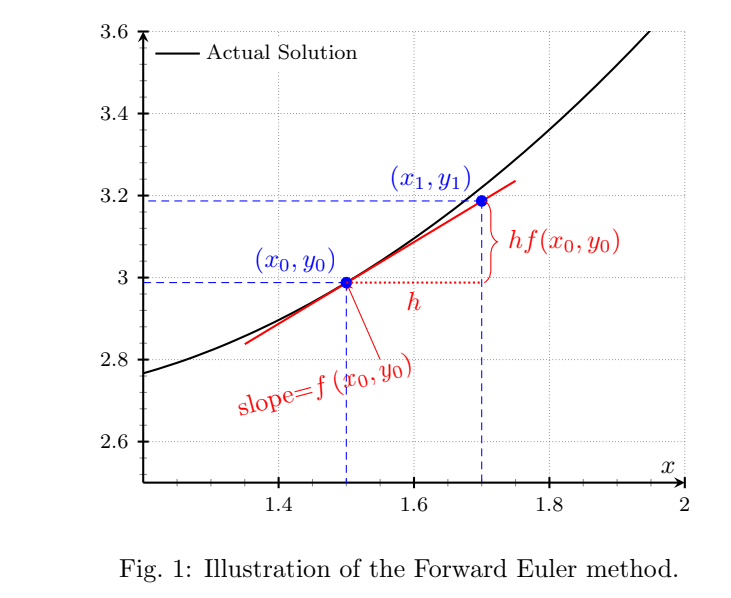
\includegraphics[width=0.8\textwidth]{fig1.png}
\end{figure}
\newpage
We know , $x_1 = x_0 + h$ \\
\\
Then clearly $ y_1 = y_0(\textbf{previous value}) + hf(x_0,y_0)(\textbf{increment in x*slope}) $ is the new updated value \\
\\
This is done iteratively to get further values and hence we can graph them.\\ 

\section*{BACKWARD EULER METHOD}

Backward euler method is very similar to forward . In simpler terms we can say that Forward Method is explicit while backward is implicit \\
\\
In forward method we update equation by using an increasing slope equation evident from above while in backward we use the decreasing slope by putting the new coordinates into slope i.e. using an unknown slope to find the new coordinates.\\ 
\\
The following figure could help with the query.
\begin{figure}[h!] % Another figure
  \centering
  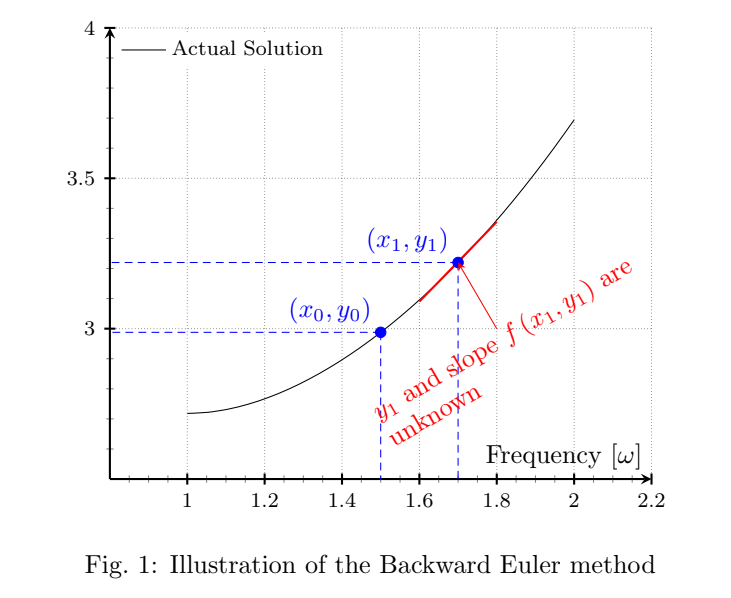
\includegraphics[width=0.8\textwidth]{fig2.png}
\end{figure}
\newpage
From the figure, We can say that the equation is being updated as to by a take back equation\\
Here, We can say $y_0 = y_1 - hf(x_1,y_1)(\textbf{decrease in x * slope at that point})$ as $x_0 = x_1 - h $ \\
\\
Now we can write the equations for updated points as 
\begin{align*}
    x_1 &= x_0 + h \\ 
    y_1 &= y_0 + hf(x_1,y_1)
\end{align*}
This process is done iteratively and for any $n_{th}$ iterative step, the updating difference equation would be as follows  
\begin{align*}
    x_{n+1} &= x_n + h \\ 
    y_{n+1} &= y_n + hf(x_{n+1},y_{n+1})
\end{align*}
And similar to forward we can find the points and plot them to get the graph of the original equation.\\
\\
\section*{Solving the problem}
Now consider the following problem\\
Find the response of LR circuit where $v(t)$ varies as follows
\begin{figure}[h!] % Another figure
  \centering
  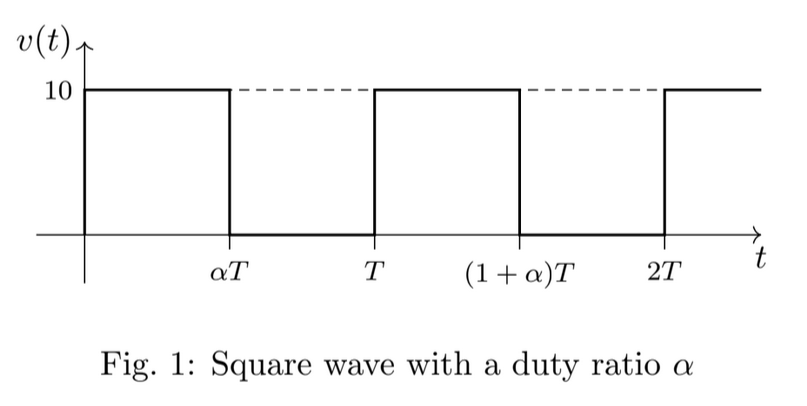
\includegraphics[width=0.8\textwidth]{fig3.png}
\end{figure}
\newpage
\textbf{Solution}\\
\\
$v(t)$ can be written as
\begin{align*}
    v(t) =
\begin{cases}
10 & \text{if } nT < t < (n+1)\alpha t \\
0 & \text{if } (n+1)\alpha T < t < (n+1)T 
\end{cases}
\end{align*}
Considering $R=1$, $L=1$ and $T=2$
\section*{CODE}
\begin{lstlisting}
import numpy as np
import matplotlib.pyplot as plt

V = 10.0  
dt = 0.001  

def squarewave(t, T, alpha):
    return V if (t % T) < (alpha * T) else 0

def euler(R, L, alpha, T):
    steps = int(duration / dt)
    i = 0.0
    tau = L / R
    time, currents = [], []

    for n in range(steps):
        t = n * dt
        v = squarewave(t, T, alpha)
        di = (v - R * i) / L
        i += dt * di
        time.append(t)
        currents.append(i)

    return time, currents

def backeuler(R, L, alpha, T):
    steps = int(duration / dt)
    i = 0.0
    tau = L / R
    time, currents = [], []

    for n in range(steps):
        t = n * dt
        v = squarewave(t, T, alpha)
        if v == V:
            i = (i + (dt * v / L)) / (1 + (dt * R / L))
        else:
            i *= np.exp(-dt / tau)
        time.append(t)
        currents.append(i)

    return time, currents

R = 1.0
L = 1.0
#alpha = 0.2
#alpha = 0.5
#alpha = 0.8
T = 2.0
duration = 4.0  

timeeuler, currentseuler = euler(R, L, alpha, T)
timebackeuler, currentsbackeuler = backeuler(R, L, alpha, T)

plt.plot(timeeuler, currentseuler, label='Euler Method')
plt.plot(timebackeuler, currentsbackeuler, '--', label='Backward Euler Method')
plt.xlabel('Time (s)')
plt.ylabel('Current (A)')
plt.title('RL Circuit Response to Square Wave')
plt.legend()
plt.grid(True)
plt.savefig("fig.png")
plt.show()
\end{lstlisting}

\begin{figure}[h!] % Another figure
  \centering
  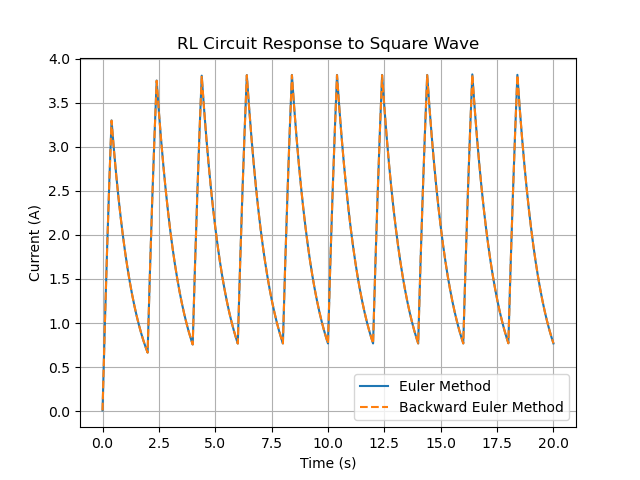
\includegraphics[width=0.8\textwidth]{fig(0.2).png}
  \caption{$\alpha = 0.2$}
\end{figure}

\begin{figure}[h!] % Another figure
  \centering
  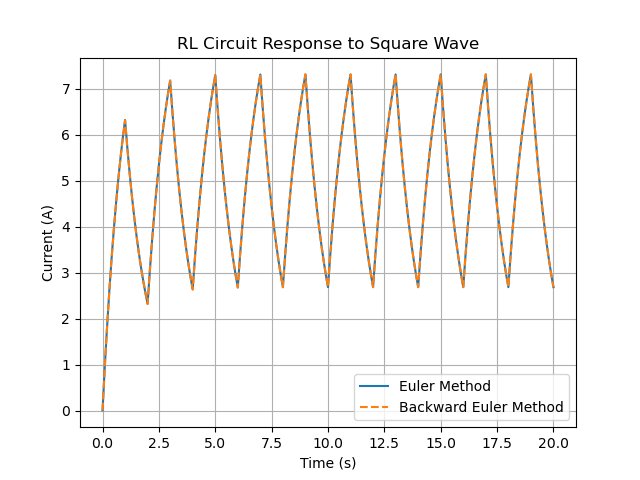
\includegraphics[width=0.8\textwidth]{fig(0.5).png}
  \caption{$\alpha = 0.5$}
\end{figure}

\begin{figure}[h!] % Another figure
  \centering
  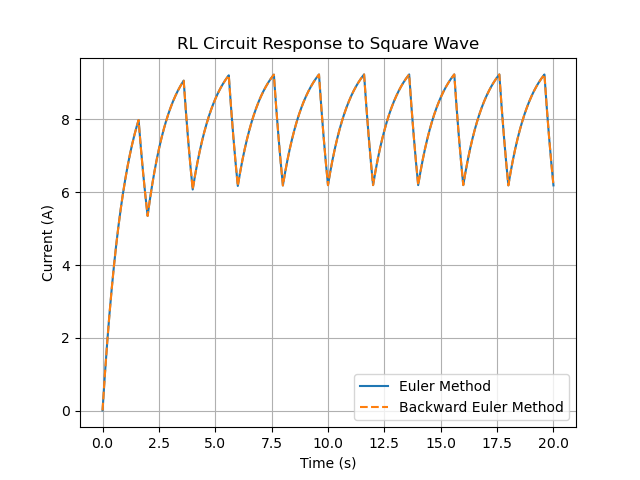
\includegraphics[width=0.8\textwidth]{fig(0.8).png}
  \caption{$\alpha = 0.8$}
\end{figure}


\end{document}

